\documentclass[letterpaper]{article}
% DO NOT CHANGE THIS
% \usepackage[submission]{aaai23} % DO NOT CHANGE THIS
\usepackage[submission]{../AuthorKit23/AnonymousSubmission/LaTeX/aaai23}
\usepackage{times} % DO NOT CHANGE THIS
\usepackage{helvet} % DO NOT CHANGE THIS
\usepackage{courier} % DO NOT CHANGE THIS
\usepackage[hyphens]{url} % DO NOT CHANGE THIS
\usepackage{graphicx} % DO NOT CHANGE THIS
\urlstyle{rm} % DO NOT CHANGE THIS
\def\UrlFont{\rm} % DO NOT CHANGE THIS
\usepackage{graphicx} % DO NOT CHANGE THIS
\usepackage{natbib} % DO NOT CHANGE THIS
\usepackage{caption} % DO NOT CHANGE THIS
\frenchspacing % DO NOT CHANGE THIS
\setlength{\pdfpagewidth}{8.5in} % DO NOT CHANGE THIS
\setlength{\pdfpageheight}{11in} % DO NOT CHANGE THIS
%
% Keep the \pdfinfo as shown here. There’s no need
% for you to add the /Title and /Author tags.
\pdfinfo{
	/TemplateVersion (2023.1)
} 
\usepackage{booktabs} 
\usepackage[ruled, noend, linesnumbered]{algorithm2e}  
\usepackage{csquotes}
\usepackage{subcaption}
\usepackage{amssymb,amsmath}
\usepackage{todonotes} 
\usepackage{tikz}

\newtheorem{theorem}{Theorem}
\newtheorem{proof}{Proof}

\newcommand{\Eff} {\ensuremath{\mathit{eff}}}  % example command without arguments
\newcommand{\Pre} {\ensuremath{\mathit{pre}}}  % (again)

\newcommand{\Add} {\ensuremath{\mathit{add}}}
\newcommand{\Del} {\ensuremath{\mathit{del}}}
\newcommand{\PreS} {\ensuremath{\mathit{pre^{*}}}}
\newcommand{\AddS} {\ensuremath{\mathit{add^{*}}}}
\newcommand{\DelS} {\ensuremath{\mathit{del^{*}}}}
\newcommand{\singlePrec} {\ensuremath{\mathit{ \mathord{\prec} }}}
\newcommand{\tasks} {\ensuremath{\mathit{tasks}}}

\newcommand{\EffPlus} {\ensuremath{\mathit{eff^{+}_{*}}}}
\newcommand{\EffMinus} {\ensuremath{\mathit{eff^{-}_{*}}}}
\newcommand{\PossEffPlus} {\ensuremath{\mathit{poss-eff^{+}_{*}}}}
\newcommand{\PossEffMinus} {\ensuremath{\mathit{poss-eff^{-}_{*}}}}

\newcommand{\RelEffPlus} {\ensuremath{\mathit{eff^{\emptyset +}_{*}}}}
\newcommand{\RelEffMinus} {\ensuremath{\mathit{eff^{\emptyset -}_{*}}}}
\newcommand{\RelPossEffPlus} {\ensuremath{\mathit{\textit{poss-eff}^{\emptyset +}_{*}}}}
\newcommand{\RelPossEffMinus} {\ensuremath{\mathit{\textit{poss-eff}^{\emptyset -}_{*}}}}

\title{Transforming Partially Ordered HTN Problems to Totally Ordered}
\begin{document}
\maketitle

\begin{abstract}
Solving partially ordered hierarchical planning problems is more computationally expensive compared to solving totally ordered ones. Therefore, automatically transforming partially ordered problem domains into totally ordered ones, such that the totally ordered problem still retains at least one solution, would be a desired capability as it would reduce complexity and thus make it easier for planning systems to solve the problem. It also allows the planner to use algorithms and heuristics specialised for the totally ordered case to solve the transformed problem. 

This is a complex endeavour, and not even possible in some cases, because even creating \emph{all} possible linearizations of all methods in the original domain does not guarantee that solutions are preserved. 

In this paper, we propose an algorithm for converting partially ordered problems into totally ordered ones and give criterion for when this conversion will retain at least one solution. We test our techniques on the partially-ordered track of the bench-mark set of the IPC 2020 and solve both the linearized and the original partially-ordered problems using state-of-the-art planning systems. We find that in the majority of problems across a variety of domains, the linearized problems remain solvable, and can always be solved faster than the without our proposed pre-processing technique. We can thus conclude our proposed pre-processing technique becomes (part of)
the state of the art for solving partially ordered planning problems.
\end{abstract}

\section{Introduction}
 
Hierarchical Task Network (HTN) planning is a hierarchical approach to planning. As defined by \cite{HTNSurvey},  %  and \cite{IntroGhallab},
tasks in HTN planning are either primitive, corresponding to an action that can be taken, or compound. HTN problems have a set of methods that specify how one might achieve a given compound task, by decomposing it into a set of sub-tasks. A compound task may even decompose into itself, either directly via a method, or indirectly via a sequence of method applications. If decomposition leads to a sequence of primitive tasks executable from the initial state, then this sequence of actions is a solution to the problem, also known as a \enquote{plan}. 
 
In totally ordered HTN planning, or TOHTN planning, methods specify a total order on the sub-tasks. In partially ordered HTN planning, or POHTN planning, methods might only specify a partial order on the sub-tasks. 

Certain kinds of problems might be naturally more suited to being modelled as a partially ordered problem, for example, the actions \enquote{deliver package 1 to city A} and \enquote{deliver package 2 to city B} -- these are essentially unrelated goals in a real transport scenario, and so modelling the problem to require that one task be completed before the other would be unnecessarily limiting the possible solution space. For some problems, such over-specification may remove all valid solutions. Thus many problems might be \emph{modelled} as POHTN problems. However, for \emph{solving} the problem, it is desirable to have additional constraints that reduces the search space, while still preserving at least some of the actual solutions. In particular, TOHTN planning as a class of problems has lower computational complexity than POHTN planning, as proven by \cite{ErolHTNExpressivity}, resulting in lower worst-case solving time. Converting the problem to a TOHTN problem allows us to exploit that fact to solve the problem more quickly.

Another benefit of transforming a POHTN problem to a TOHTN problem is that the additional structure to the problem could allow us to deploy specialised algorithms and heuristics for the totally ordered case. Also, heuristic design is comparably easy for total-order problems due to the missing interaction between tasks.

The drawback to this approach is that, due to the greater expressivity of POHTN planning, there may exist POHTN problems that cannot be solved when converted to a TOHTN problem. For example, \cite{ErolHTNExpressivity} proved that POHTN planning is expressive enough to model undecidable problems, such as the language intersection problem of two context-free languages. On the other hand, TOHTN planning is not expressive enough to model undecideable problems. Fortunately, not every POHTN problem is guaranteed to be undecidable, and so could still be transformed while preserving at least one solution.

% Also, we get another class of decidable partially ordered problems that's orthogonal to recursive ones. 
% Also, the domain model might be more intuitive: if a task is independent of some others it might be counter-intuitive to demand a certain position of it (if artificially made totally ordered). Plan recognition: independent goals can be described in parallel with POHTN planning but not with TOHTN, as per \cite{DanielPlanRecognition}.

%\subsubsection{Contributions}
%Gregor Behnke used a similar linearization process to produce the TO benchmark set used for the 2020 International Planning Competition (IPC 2020). That also attempted to linearize the methods by drawing the same links between preconditions and effects as in this paper, and picked a random linearization if that was not possible. However, no attempt was made to analyse if this lead to a easier to solve problem, or if it had any interesting theoretical implications. As Prof. Bercher thought this could be an interesting use for linearization, this paper offers this empirical evaluation and theoretical analysis.

In this paper we present and investigate an algorithm for converting POHTN problems to TOHTN problems. We prove that when certain criteria are met, it guarantees that at least one solution will be preserved. 
Also, we obtain a new class of decidable problems, namely those that satisfy the above mentioned criterion. Finally, we show that, even when these criteria are not met, very few problems are rendered unsolvable by the transformation, and that it greatly reduces solving time for problems, with gains being bigger for more difficult problems. 


\section{Hierarchical Planning Formalism}
Hierarchical task network planning, also known as \textbf{HTN planning}, is one form of hierarchical planning. There are many formalisations for HTN planning. The following one borrows heavily from \cite{HTNSurvey} and \cite{Geier2011TIHTNDecidability}. HTN planning can be partially ordered, also known as POHTN planning, or totally ordered, otherwise known as TOHTN planning. TOHTN planning is a special case of POHTN planning.  % except with the initial task network replaced by a initial compound task. 

A \textbf{Partially Ordered Hierarchical Planning}(POHTN) problem \textbf{P} = $(D, S_I, T_I)$
is defined over some domain $D$, 
has an initial state $S_I \in 2^F$, and 
has a initial compound task $T_I$. 
The closed world assumption also holds for HTN planning.

The domain is defined as \textbf{D} = $(F, T_P, T_C, \delta, M)$.
$F$ is the finite set of facts or state variables, $T_P$ is the finite set of all possible primitive task names, $T_C$ is the finite set of all possible compound task names, and
$\delta$ is a mapping from primitive task name to action. Actions in POHTN domain also have preconditions, adds, and delete effects.
$M$ is the finite set of decomposition methods. Each one maps a compound task name to a task network. If $m \in M$, then $m=(c, tn)$, where $c \in T_C$.

A task network \textbf{tn} = $(T, \singlePrec, \alpha)$ consists of
T, which is a finite set of task identifiers (ids); 
$\singlePrec$, which is a partial order over T; and
$\alpha$, which maps task ids $\in$ T to task names in $T_C$ and $T_P$. 

% replacing t  (i.e. $tn_1 \rightarrow_{t,m} tn_2$)
A method $m = (c, tn_m)$ decomposes a task network $tn_1 = (T_1, \singlePrec_1, \alpha_1)$ into
a new task network $tn_2$ by replacing $t$, if and only if $t \in T_1$, $\alpha_1(t) = c$, and $\exists tn' = (T', \singlePrec' \alpha')$ with $tn' \cong tn_m$ and $T' \cap T = \emptyset$ and
\begin{align}
tn_2 :=     &((T_1 \setminus \{t\}) \cup T',    \singlePrec_1 \cup \singlePrec' \cup \singlePrec_X,        \alpha_1 \cup \alpha') \\
\singlePrec_X :=  &\{(t_1, t_2) \in T_1 \times T'  \mid  (t_1,t) \in \singlePrec_1 \} \cup \\
&\{(t_1, t_2) \in T' \times T_1 \mid (t, t_2) \in \singlePrec_1 \}  
\end{align}
In other words, the decomposition of a compound task results in it being removed from the task network and replaced by a copy of the method’s task network. The ordering constraints
on the removed task are inherited by its replacement tasks, as defined by $\singlePrec_X$. 

A \textbf{solution} to an HTN problem is a task network $tn = (T, \prec, \alpha)$ if and only if
tn can be reached via decomposing $tn_I$, all tasks are primitive, ($\forall t \in T: \alpha(t) \in T_P$), and there exists a sequence $\langle t_1, t_2 ... t_n \rangle$ of the task ids in $T$ that agrees with $\prec$ such that the application of that sequence $\langle \alpha(t_1), \alpha(t_2) ... \alpha(t_n) \rangle$ in $S_I$ is executable.

In other words, there is no goal state for hierarchical planning -- the goal is to find an decomposition of the initial task, then any executable refinement of the resulting decomposition. For any given hierarchical problem, it is trivial to enforce a goal state is met, by replacing the real initial task with a task whose only decomposition is to the real initial task and a primitive task ordered after it whose preconditions are equivalent to any \enquote{goal state} desired. Thus the fact that a goal state is not strictly required is not a restriction to the expressiveness of hierarchical planning. Whereas in classical planning, one only finds any executable sequence of actions to achieve a goal state, so HTN planning poses additional restrictions on which action sequences may be considered.


\textbf{Totally Ordered Hierarchical Planning}, also called TOHTN planning, is the same as partially ordered planning in all respects except the kind of task networks it allows.
For both planning formalisms, a method $m$ maps a task $t$ to a task network \textbf{tn} = $(T, \prec, \alpha)$. TOHTN planning domains require that $\prec$ must specify a total order between task ids in $T$.
This leads to a difference in expressiveness and decideability of TOHTN vs POHTN planning. POHTN planning is more expressive in general (both in terms of plan existence and in terms of computational complexity). As per \cite{LanguageClassificationPlanning}, if regarded from the standpoint of formal grammars, TOHTN planning is exactly as expressive as context free languages, whereas POHTN planning is strictly more expressive than context-free languages, and strictly less expressive than context-sensitive languages.
In terms of complexity classes, \cite{ErolHTNExpressivity} proved that POHTN planning is semi-decidable, whereas \cite{Alford2015TightHTNBounds} proved that, assuming arbitrary recursion, TOHTN planning is 2-EXPTIME-complete with variables, and EXPTIME-complete without. 


\section{Simple Linearization Procedure}
The basic linearization process consists of inferring preconditions and effects for compound tasks, inferring additional orderings to the sub-tasks based on the preconditions and effects (inferred or \enquote{real} in the case of primitive tasks) of method sub-tasks, and adding them only if they do not conflict with the originally required orderings.

For a lifted domain, where a predicate $f$ accepts parameters $p_1, ..., p_n$, 
$f' = f(o_1, ..., o_n)$, where $o_1, ..., o_n$ are arbitrary objects of the appropriate type. For a grounded model, $f' = f$. The inferred preconditions and effects for a task are then defined as below:
\begin{align*}
& \forall t \in T_P : \PreS(t) := \Pre(t) \\
& \forall t \in T_P : \AddS(t) := \Add(t) \\
& \forall t \in T_P : \DelS(t) := \Del(t)  \\ %  \land
& \forall t \in T_C : \PreS(t) := \{f'  \mid  \exists m \in M  \\
								& : m=(t,(T, \singlePrec, \alpha)) \forall t' \in T.  \forall  f \in \PreS(t') \}   \\
& \forall t \in T_C : \AddS(t) := \{f'  \mid  \exists m \in M : \\
								& m=(t,(T, \singlePrec, \alpha)) \forall t' \in T.  \forall  f \in \AddS(t') \}   \\
& \forall t \in T_C : \DelS(t) := \{f'  \mid  \exists m \in M : \\
								& m=(t,(T, \singlePrec, \alpha)) \forall t' \in T.  \forall  f \in \DelS(t') \}   \\ 
\end{align*}
 
From these inferred preconditions and effects $\PreS(t), \AddS(t), \DelS(t)$, (which may have been derived using the ground or lifted variant), we can run Algorithm~\ref{alg:Algorithm1}.

\begin{algorithm}\label{alg:Algorithm1}
	\KwData{$(F, T_P, T_C, \delta, M)$}
	\KwResult{$(F, T_P, T_C, \delta, M)$}
	
	\For {$m=(t, (T_m, \singlePrec, \alpha)) \in M$} 
	{
		
		\tcc{An edge $(t, t')$ in $G$ means $t$ is ordered before $t'$}  
		
		$G \gets$ calculateTransitiveClosure($\singlePrec$) \\
		\label{alg:StartBuildGraph}
		\For{a $\in$ F}{  
			\For{$t \in T_m$}{
				\For{$t' \in T_m$}{
					if $a \in \AddS(t)$ and $a \in \PreS(t')$, and $(t', t)$ not in $G$, add $(t, t')$ to $G$  \\ 
					if $a \in \AddS(t)$ and $a \in \DelS(t')$, and $(t, t')$ not in $G$, add $(t', t)$ to $G$  \\ 
					if $a \in \DelS(t)$ and $a \in \PreS(t')$, and $(t, t')$ not in $G$, add $(t', t)$ to $G$  \\ 
					if $a \in \DelS(t)$ and $a \in \AddS(t')$, and $(t', t)$ not in $G$, add $(t, t')$ to $G$ \\  
				}
			} 
			\label{alg:EndBuildGraph}	
		}	 
		\label{alg:TopSort}
		$\singlePrec'\gets$ any linearization of $G$ \\
		$m' = (tasks(m), \singlePrec', \alpha(t))$ \\
		$M' = M' \cup  \{m'\}$ \\		
	}
	\Return $D' = (F, T_P, T_C, \delta, M')$ \\
	\caption{Calculation of linearized methods}
\end{algorithm}

\subsection{Theoretical Properties of Linearization Result}
\begin{theorem}\label{thm:Runtime}
	Given a problem $P = (F, T_P, T_C, \delta, M)$, Algorithm~\ref{alg:Algorithm1} takes at most quadratic time, $\mathcal{O}( |M| * |F| * |T|^2)$. 
\end{theorem}
\begin{proof}  % ,  network of tasks it can decompose to as a tree of tasks whose edges are between a task and a task it can decompose to, since it excludes previously seen tasks. 
	Let $|T|$ = $|T_P| + |T_C|$.
	
	The Floyd-warshall algorithm to calculate transitive closure is used for each method's sub-tasks, resulting in a time complexity of $\mathcal{O}(|M| * |T|^3)$, 

		
	To calculate $\PreS, \AddS, \DelS$ for each task $t$, we can perform breadth-first search on the task decomposition sub-tree (where tasks are nodes, and edges indicate possible decomposition by methods) rooted at $t$. The size of a sub-tree has an upper limit of $T_C + T_P$ nodes. For each primitive task in the sub-tree, we can iterate over each fact to update $\PreS, \AddS, \DelS$ for the root $t$. Thus calculating  $\PreS, \AddS, \DelS$ for a single compound task has an upper limit of $(3 * |F| * |T_p|) + |T_C|$. This inference occurs for each compound task, so inference for all compound tasks takes $((3 * |F| * |T_P|) + |T_C|) * |T_C|$ time at most, or $\mathcal{O}(|F| * |T|^2)$.
	
	Lines~\ref{alg:StartBuildGraph}-\ref{alg:EndBuildGraph} of Algorithm~\ref{alg:Algorithm1} iterates over every method, which iterates over every fact, which iterates over every sub-task in that method, which iterates over every other sub-task in that method. Leading to $(M * F * (t_m)^2)$, where $t_m$ is the average number of sub-tasks per method. So it's at most $\mathcal{O}(|M| * |F| * |T|^2)$, since $t_m$ has an upper bound of $T$, where $T=T_p + T_C$.		

	Line~\ref{alg:TopSort} can be done via topological sort of the graph (which is known to be in $\mathcal{O}(V+E)$ in time and $\mathcal{O}(V)$ in space). In this case, the nodes of the graph are tasks, and the edges are orderings. So that's $M * (t_m+e_m)$, where $e_m$ is the number of \enquote{edges} in the new method, and has an upper bound of $e_m$ to find a topological sort for the sub-tasks of every method. That's approximately $\mathcal{O}(|M| * |T|)$, since both $t_m$ and $t_e$ are upper bounded by $T$, such that $T=T_p + T_C$.
	
	So in total the main algorithm takes: \newline
	$(|M| * |T|^3)$ +          % Floyd-Warshall
	$(|M| * |F| * |T|)$  +    % GetPreEff
	$\mathcal{O}(|M| * |F| * |T|^2)$ +  % desired orderings
	$(|M| * |T|)$        % topological sort
\end{proof}


\begin{theorem}\label{thm:Soundness}
	Given a POHTN planning problem $P$ and TOHTN problem
	$P'$ obtained from $P$ by using Algorithm~\ref{alg:Algorithm1}
	then the solution set of $P'$, denoted $sol(P')$ is a strict subset of $sol(P)$.
\end{theorem}
\begin{proof}
	The new desired orderings for a method include all of the orderings already required by the method originally. The algorithm then turns the tasks and new desired orderings between them into a directed graph, and the new ordering is produced by performing a topological sort on the nodes of that graph. This means we do not modify the sub-tasks a method produces, just the ordering between them, so the set of plans from the totally ordered method is just a subset of the plans possible from the partially ordered one. Any solution to the linearized problem is then obviously a solution to the original problem.
\end{proof}


\begin{theorem}\label{thm:notCompleteness}
	Given a POHTN planning problem $P$ and TOHTN problem
	$P'$ obtained from $P$ by using Algorithm~\ref{alg:Algorithm1}
	then $sol(P')$ may be empty.
\end{theorem}
\begin{proof}
	This algorithm linearizes all the methods to be totally ordered. Since sub-tasks inherit the orderings of their parents, it's impossible to preserve a solution that requires the interleaving of sub-tasks if their respective parents that are already ordered with respect to each other. This proves that the algorithm can remove some possible action sequences, assuming the original domain was not already totally ordered. Consider the simple example problem:
	
	
	\begin{figure}
		\caption{Diagram showing an example problem and its decomposition.}		
		\begin{subfigure}{3.5cm}
			\begin{align*}
			F   = & \{a, b, c \}           \\
			N_p = & \{A, B, C\}      \\
			N_c = & \{AC, T_I\}            \\ 
			M   = & \{  (T_I, \{AC, B\}), \\
			&    (AC, \{A, C\})  \} \\
			S_I = & \{ a \} 	             \\ 
			\end{align*} 
		\end{subfigure}		
		\scalebox{0.7}{
			\begin{subfigure}{7cm}
				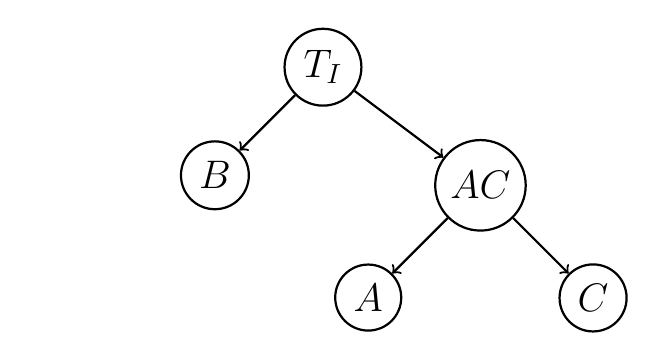
\begin{tikzpicture}[auto,node distance=1.5cm,
				thick,main node/.style={circle,draw,font=\sffamily\Large\bfseries},
				square node/.style={rectangle,draw,font=\sffamily\Large\bfseries}]
				\node[] (InitState) {}; %{ $\mathbf{S_I = \{a\}}$ };
				
				\node[main node] (Init) [right=3cm of InitState] {$T_I$};
				\node[main node] (AC) [right=2cm of Init, below of=Init] {$AC$}; 
				
				\node[main node] (A) [below left = 2em and 2em of AC] {$A$};
				\node[main node] (B) [below left = 2em and 2em of Init] {$B$}; 
				\node[main node] (C) [below right = 2em and 2em of AC] {$C$}; 
				
		%		\action{A}{PrimitiveA,
		%			width  = 2.5em, 
		%			height = 2.5em, 
		%			pre length = 2em,
		%			eff length = 2em,
		%			body = {below left = 2em and 2em of AC} 
		%		};			
				
		%		\action{B}{PrimitiveB,
		%			width  = 2.5em, 
		%			height = 2.5em, 
		%			pre length = 2em,
		%			eff length = 2em,
		%			body = {below left = 2em and 2em of Init} 
		%		};
				
		%		\action{C}{PrimitiveC,
		%			width  = 2.5em, 
		%			height = 2.5em, 
		%			pre length = 2em,
		%			eff length = 2em,
		%			body = {below right = 2em and 2em of AC} 
		%		};
				
				\path[every node/.style={font=\sffamily\small}]
				(Init) edge [->] node [left] {} (B)
				(Init) edge [->] node [left] {} (AC)
				(AC) edge [->] node [left] {} (A)
				(AC) edge [->] node [left] {} (C);
				\end{tikzpicture}
			\end{subfigure}	
		}
	\end{figure}
	
	\begin{figure}
		\caption{The only possible solution $A, B, C$ for E.g.\ 1, requires the children of $AC$ and $B$ to be interleaved, meaning we cannot impose an order between them}
		\scalebox{0.9}{
			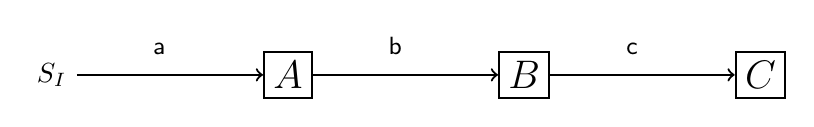
\begin{tikzpicture}[auto,node distance=3cm,
			thick,main node/.style={circle,draw,font=\sffamily\Large\bfseries},
			square node/.style={rectangle,draw,font=\sffamily\Large\bfseries}]
			
			\node[] (Invis) [] {$S_I$};
			\node[square node] (A) [right of=Invis] {$A$};
			\node[square node] (B) [right of=A] {$B$};
			\node[square node] (C) [right of=B] {$C$};
			
			
			\path[every node/.style={font=\sffamily\small}]
			(Invis) edge [->] node [left, label=a] {} (A)
			(A) edge [->] node [left, label=b] {} (B)
			(B) edge [->] node [left, label=c] {} (C);
			\end{tikzpicture}		
		}
	\end{figure}
	
	The only decomposition for this problem results in the set of un-ordered actions $\{A, B, C\}$.
	If we consider that for the $3!$ linearizations of this set, the only executable one is $A, B, C$. This is impossible to achieve by linearized methods, since ordering either AB before C or C before AB will exclude the solution. 
	Even if we were to produce $k!$ methods for each partially ordered method with $k$ unordered sub-tasks, we would not be able to preserve any solution for this problem.
	
	This proves that the algorithm can remove all solutions, so Algorithm~\ref{alg:Algorithm1} is not complete. Note that incompleteness already follows from complexity theory as it's theoretically impossible to turn an arbitrary undecidable problem into a decidable one.
	Specifically, solutions that require interleaving of sub-tasks will not be preserved, as the example above demonstrates.
\end{proof}

We will now see that our algorithm preserves at least one solution as long as Algorithm~\ref{alg:Algorithm1} does not have to break cycles.
\begin{theorem}\label{thm:SpecialCase}
	Given a POHTN planning problem $P$ and TOHTN problem
	$P'$ obtained from $P$ by using Algorithm~\ref{alg:Algorithm1}, if Algorithm~\ref{alg:Algorithm1} did not have to
	cycle-break, then if $sol(P)$ is non-empty then $sol(P')$, will be non-empty as well.
\end{theorem}
\begin{proof}
	Assume that there exists a solution in the PO domain. By using the same decomposition sequence in the linearized domain, we can produce the same set of actions as in the PO solution, but with a linearization of the actions decided by the linearized domain. Assume this sequence is $(a_0, a_1, ..., a_n)$. We then prove by induction over the sequence $(a_0, a_1, ..., a_n)$ that it is executable.
	If $(a_0, a_1, ..., a_n)$ is not executable, that means there exists some action $a_k,  0 < k < n$ that is not executable in the corresponding state. The action $a_k$ could only be non-executable, if one or more of its preconditions was not met. Assume one of these unmet preconditions is for existence of the state variable $A$.
	The action $a_k$ must be executable in some linearization of $\{a_0, ..., a_n\}$, as we assumed it was a PO solution. So there must exist an action $a_i$, $0 < i < n$, that will add A. Actions $a_0$ and $a_k$ must have a shared parent p in a Task Decomposition Tree. So p has subtasks $t_0$ and $t_k$ that are parents of $a_0$ and $a_k$ respectively. 
	
	The linearization of this method would have drawn an ordering $(t_i, t_k)$ due to the way the algorithm defines $prec^{*}, add^{*}$ etc. We are assuming that all methods linearized without conflict, so $(t_i, t_k)$ should not be required. This safely enforces $(a_k, a_0)$ ordering in the final TO plan, meaning $a_0$ is not the first action in the resulting total order imposed by the algorithm. In other words, if $a_k$’s precondition could be met by any action $a_i$, $a_i$ would be ordered in front of it. 
	
	If $a_i$ does not exist then $a_k$ can never be executed for any linearization of $\{a_0, ...a_n\}$, contradicting the assumption that this was a PO solution. Since each action in the solution is executable, the entire sequence is executable linearization of actions produced by decomposition of initial task, i.e.\ the solution.
\end{proof}

There are several possible levels of \enquote{completeness} for a problem compilation.
%\begin{enumerate}
\begin{itemize}
	\item all solutions remain 
	\item at least one solution remains 
	\item all optimal solutions remain
	\item at least one optimal solution remains 	
\end{itemize}
%\end{enumerate}
Given what's proven in Theorem~\ref{thm:notCompleteness} and \ref{thm:SpecialCase}, Algorithm~\ref{alg:Algorithm1} guarantees at least one solution remains, if no cycle-breaking is needed. If cycle-breaking is needed, Algorithm~\ref{alg:Algorithm1} makes no completeness guarantees at all -- it may remove all possible solutions. Finally, Algorithm~\ref{alg:Algorithm1} makes no decisions on any metric of optimality, so obviously cannot guarantee completeness that any optimal solutions remain.


\begin{theorem}\label{thm:newClass}
	Problems $P$ that satisfy the criterion for linearization without cycle-breaking form a new class of decidable problems.
\end{theorem}
\begin{proof}
	A problem $P'$ obtained from applying Algorithm~\ref{alg:Algorithm1} to any arbitrary $P$ is a totally ordered problem, which are known to be decidable, as proven by \cite{Alford2015TightHTNBounds}.  
\end{proof}






\section{Complex Linearization Procedure}

The work by \cite{ConnyPreEff}, details a way to infer a subset of the mandatory preconditions and effects.

\emph{Mandatory preconditions} of a compound task $c$ are facts that hold in every state for which there exists an executable refinement. So, they are required in every state in which a refinement of c shall be executed: prec(c) := $\cap_{s \in E(c)}  s$
if $E(c) \neq \emptyset and prec(c) := undef$ otherwise.

State-independent positive and negative effects (cf. their
Def. 4) of a compound task c are facts that are added or
deleted, resp., by the successful execution of a refinement of
c, independent of the state in which the task is executed, i.e.
$$ \RelEffPlus := ( \bigcap_{s \in E(c)} \bigcap_{s' \in R_s(c)} s') \backslash  \bigcap_{s \in E(c)} s    $$
$$ \RelEffMinus := \bigcap_{s \in E(c)}  (F \backslash \bigcap_{s' \in R_s(c)} s' ) $$

Possible state-independent effects of a compound task $c$ are not guaranteed to hold (or not hold, resp.,)
after every refinement of c but after at least one:
$$ \RelPossEffPlus(c) := \bigcup_{s \in E(c)}  ( \bigcup_{s' \in R_s(c)}  s' \backslash s) $$
$$ \RelPossEffMinus(c) := \bigcup_{s \in E(c)} ((\bigcup_{s' \in R_s(c)} (F \backslash s') \cap s ))$$
if $E(c) \neq \emptyset and prec(c) := undef$ otherwise.


The set of executability-enabling states of c is
$E(c) = \{s \in 2F  \mid  \exists \text{t.o. refinement of c applicable in s} \}$.
The set of resulting states of c w.r.t. some state $s \in 2^F$ is
$R_s(c) = \{s' \in 2^F | \exists t.o. refinement appl. in s res. in s' \}$.

So, the precondition-relaxation of a domain D = $(F, A, C, M)$ is the domain $D' = (F, A', C, M)$
with $A' = \{(\emptyset, add , del ) \mid (prec, add , del ) \in A\}$.
Then, the precondition-relaxed effects $\RelEffPlus$, $\RelEffMinus$, $\RelPossEffPlus$, $\RelPossEffMinus$. are defined
just like the original ones but based on the precondition-
relaxed variant of D.
 
We can use these as an alternative input to Algorithm~\ref{alg:Algorithm1}.




\section{Empirical Evaluation}

To prove that our technique improves the solving time, we compare the runtime of a state-of-the-art planning system on the original problem vs. the transformed problem, for a number of different PO domains. All problems are taken from two benchmark sets prepared for the International Planning Competition (IPC) 2020. The first set \footnote{https://github.com/panda-planner-dev/ipc2020-domains/tree/master/partial-order} was used in the partially ordered track in the 2020 IPC benchmark, while the second set \footnote{https://github.com/panda-planner-dev/domains/tree/master/partial-order} went un-used for various reasons. Each problem has the standard IPC time limit of 30 minutes. Any grounding and pre-processing time needed is included as part of the 'solving' time. Since the pre-processing may \emph{potentially} remove all solutions, where the planning system can prove that the pre-processing renders a problem unsolvable, we use the remaining time to solve the original problem, called a \textit{re-run}.

\subsection{Hardware and Planning Systems}
The empirical evaluation was conducted on a machine with 30GiB of memory and 4 vCPUs, each with 2 GiB RAM. Recent work by \cite{HTN2SAS} shows that the partial-order panda$_\pi$, actually achieved similar coverage and slightly lower IPC score than the best specialised TOHTN planner evaluated. %Lilotane by \cite{Lilotane} is an TOHTN solver and the IPC 2020 runner-up. The winner, HyperTensioN by \cite{hypertension} could not be tested due to lack of support for reading in optimisation metrics. 

We therefore test the $panda_{\pi}$ solver by \cite{useClassicalHuristicICAPS18,useClassicalHeuristicIJCAI19,progressionsearchJAIR20} on the configuration of Greedy best first search with visited lists, and using RC to turn the problem into a classical planning problem. We try this search with 4 different heuristics: FF by \cite{FF}, Add by \cite{Add}, Filter by \cite{useClassicalHuristicICAPS18} and Landmark-cut by \cite{LM-Cut}.

We compare the performance of these 4 planner settings on the original problem and the pre-processed problem, HTN2SAS, and the latest version of HyperTensioN and Lilotane. For panda$_{\pi}$, the same setting is used for re-runs. For TOHTN planners, re-runs use panda$_{\pi}$ on the best setting (Add heuristic). The comparison is done for grounded linearization variant and the lifted linearization variant 1.

\subsection{Performance of Simple Linearization}

\begin{table}[h]
	\scalebox{0.45} {
		\begin{tabular}{lccccccccccccccccccccccccl} 
			\toprule 
			&& \multicolumn{2}{c}{rc2(Add)} & \multicolumn{2}{c}{rc2(Filter)} & \multicolumn{2}{c}{rc2(FF)} & \multicolumn{2}{c}{rc2(LMC)}  & \multicolumn{2}{c}{HTN2SAS} & \multicolumn{2}{c}{HyperTensioN} & \multicolumn{2}{c}{Lilotane} \\ 
			\cmidrule(lr){3-4} \cmidrule(lr){5-6} \cmidrule(lr){7-8} \cmidrule(lr){9-10} \cmidrule(lr){11-12}  \cmidrule(lr){13-14} \cmidrule(lr){15-16}    
				& max &PO & TO & PO & TO & PO & TO & PO &\multicolumn{2}{c}{ TO  }   \\ 
		\midrule 
		Barman-BDI  \\ 
		Monroe Fully Observ. \\ 
		Monroe Part. Observ. \\ 
		PCP\\ 
		Rover  \\ 
		Satellite  \\ 
		Transport \\ 
		UM-Translog \\ 
		Woodworking \\ 
		\midrule 
		Monroe  \\ 
		SmartPhone \\ 
		Zenotravel \\ 
		\midrule 
		Coverage \\ 
		Norm. coverage  \\ 
		\bottomrule
			\end{tabular} 	
			}
\end{table}

\begin{table}[h]
	\scalebox{0.45} {
		\begin{tabular}{lccccccccccccccccccccccccl} 
			\toprule 
			&& \multicolumn{2}{c}{rc2(Add)} & \multicolumn{2}{c}{rc2(Filter)} & \multicolumn{2}{c}{rc2(FF)} & \multicolumn{2}{c}{rc2(LMC)}  & \multicolumn{2}{c}{HTN2SAS} & \multicolumn{2}{c}{HyperTensioN} & \multicolumn{2}{c}{Lilotane} \\ 
			\cmidrule(lr){3-4} \cmidrule(lr){5-6} \cmidrule(lr){7-8} \cmidrule(lr){9-10} \cmidrule(lr){11-12}  \cmidrule(lr){13-14} \cmidrule(lr){15-16}    
			& max &PO & TO & PO & TO & PO & TO & PO &\multicolumn{2}{c}{ TO  }   \\ 
			\midrule 
			Barman-BDI  \\ 
			Monroe Fully Observ. \\ 
			Monroe Part. Observ. \\ 
			PCP\\ 
			Rover  \\ 
			Satellite  \\ 
			Transport \\ 
			UM-Translog \\ 
			Woodworking \\ 
			\midrule 
			Monroe  \\ 
			SmartPhone \\ 
			Zenotravel \\ 
			\midrule 
			IPC \\
			\bottomrule
			\end{tabular} 	
	}
\end{table}


\subsection{Performance of Complex Linearization}

\begin{table}[h]
	\scalebox{0.45} {
		\begin{tabular}{lccccccccccccccccccccccccl} 
			\toprule 
			&& \multicolumn{2}{c}{rc2(Add)} & \multicolumn{2}{c}{rc2(Filter)} & \multicolumn{2}{c}{rc2(FF)} & \multicolumn{2}{c}{rc2(LMC)}  & \multicolumn{2}{c}{HTN2SAS} & \multicolumn{2}{c}{HyperTensioN} & \multicolumn{2}{c}{Lilotane} \\ 
			\cmidrule(lr){3-4} \cmidrule(lr){5-6} \cmidrule(lr){7-8} \cmidrule(lr){9-10} \cmidrule(lr){11-12}  \cmidrule(lr){13-14} \cmidrule(lr){15-16}    
			& max &PO & TO & PO & TO & PO & TO & PO &\multicolumn{2}{c}{ TO  }    \\ 
			\midrule 
			Barman-BDI  \\ 
			Monroe Fully Observ. \\ 
			Monroe Part. Observ. \\ 
			PCP\\ 
			Rover  \\ 
			Satellite  \\ 
			Transport \\ 
			UM-Translog \\ 
			Woodworking \\ 
			\midrule 
			Monroe  \\ 
			SmartPhone \\ 
			Zenotravel \\ 
			\midrule 
			Coverage \\ 
			Norm. coverage  \\ 
			\bottomrule
			\end{tabular} 	
	}
\end{table}

\begin{table}[h]
	\scalebox{0.45} {
		\begin{tabular}{lccccccccccccccccccccccccl} 
			\toprule 
			&& \multicolumn{2}{c}{rc2(Add)} & \multicolumn{2}{c}{rc2(Filter)} & \multicolumn{2}{c}{rc2(FF)} & \multicolumn{2}{c}{rc2(LMC)}  & \multicolumn{2}{c}{HTN2SAS} & \multicolumn{2}{c}{HyperTensioN} & \multicolumn{2}{c}{Lilotane} \\ 
			\cmidrule(lr){3-4} \cmidrule(lr){5-6} \cmidrule(lr){7-8} \cmidrule(lr){9-10} \cmidrule(lr){11-12}  \cmidrule(lr){13-14} \cmidrule(lr){15-16}    
			& max &PO & TO & PO & TO & PO & TO & PO &\multicolumn{2}{c}{ TO  }  \\ 
			\midrule 
			Barman-BDI  \\ 
			Monroe Fully Observ. \\ 
			Monroe Part. Observ. \\ 
			PCP\\ 
			Rover  \\ 
			Satellite  \\ 
			Transport \\ 
			UM-Translog \\ 
			Woodworking \\ 
			\midrule 
			Monroe  \\ 
			SmartPhone \\ 
			Zenotravel \\ 
			\midrule 
			IPC \\
			\bottomrule
		\end{tabular} 	
	}
\end{table}


As we can see, using complex inference results in ?  increase/decrease/similar, coverage and IPC score.
As we can see, the best planner is ? planner.

\section{Related Work}
% FROM (https://ojs.aaai.org/index.php/ICAPS/article/view/15944/15755) A Closer Look at Causal Links: Complexity Resultsfor Delete-Relaxation in Partial Order Causal Link (POCL) Planning
Our linearization procedure is a pre-processing technique for the search space, is a compilation of an HTN planning problem class to a different class of problems, and can exploit specialised TO planners.
 
The panda$_\pi$ grounder by \cite{Behnke2020Grounding} also prunes unreachable tasks, methods, etc.\.  Because the panda$_{\pi}$ planner is a grounded planner, we can ground then linearize, or vice-versa to \enquote{stack} the reduction in search space.

The main optimization of HyperTensioN by \cite{hypertension} is via the Pullup extension - which determines additional preconditions of methods and compound tasks by analysing the preconditions of possible child actions. Unlike ours, no approximation of effects are considered.  

The HTN2STRIPS planner by \cite{HTN2STRIPS} and HTN2SAS planner by \cite{HTN2SAS} compiles HTN problems, both totally and partially ordered, to classical problems. The TOAD planner by \cite{HollerTOAD} compiles TOHTN problems into classical planning problems in order to allow the use of classical planning systems. % TOAD over-approximates the set of solutions to the HTN problem. In the empirical evaluation the paper performed, TOAD achieved higher coverage than the base version of HTN2STRIPS, and all systems submitted to the totally ordered track of the 2020 IPC.  

There exists totSAT planner by \cite{TOtoSAT} that compiles a totally ordered problem to SAT problem. There also exists 2 planners by \cite{POtoSAT, OptimalPOtoSAT} that compiles a partially ordered problem to a SAT problem. One searches for optimal plans, the other focuses on finding any solution as quickly as possible. Lilotane by \cite{Lilotane} directly encodes a lifted problem representation into a SAT problem.

Another planner by \cite{Behnke_Speck_2021} converts TOHTN into Binary Decision Diagrams (BDDs), then use symbolic search on it.
 
The BDD planner by \cite{Behnke_Speck_2021}, totSAT planner by \cite{TOtoSAT}, TOAD by \cite{HollerTOAD}, HyperTensioN by \cite{hypertension}, and Lilotane by \cite{Lilotane}, as discussed before, are all specialised TO planners. So are the TFD (Totally Ordered Fast Downward) and PFD (Partially Ordered Fast Downward) hierarchical planners by \cite{PDDL4J}.  Note however that HTN2SAS achieved similar coverage than greedy search with panda$_\pi$, a partial-order planner.
 

\section{Summary}

The contributions of this paper are as follows:

At least for the POHTN problems in the IPC domain, most of them are not undecideable.
In another way, it is as if the POHTN domains are compressed TO domains - this linearization
separates one back out.

For another, this pre-processing technique leads to large gains in time/efficiency for a number of planners, at least for the problems tested here. Furthermore, there is demonstrably much more room for improvement. Though the criteria does not fire all the time, it's producing a linearization that is almost always solvable.

We have a method that can increase the number of TOHTN problems available for purposes like comparing TOHTN planners or grounding techniques. Suppose there were $n$ POHTN problms and $m$ TOHTN problems, and this linearization could make those $n$ POHTN problems into $k$ solvable $TOHTN$ problems. Then $k+m$ (lifted or grounded) TOHTN problems exist now. And from empirical evaluation, $k$ may be close to $n$.

We can identify a subset of decidable problems within POHTN problems, and this subset is orthogonal to all other criteria.


\section{Future Work}


\subsubsection{MAX-SAT Instead of Cycle-Break} 
The maximum satisfiability problem (MAX-SAT) is the problem of determining the maximum number of clauses, of a given Boolean formula in conjunctive normal form, that can be made true by an assignment of truth values to the variables of the formula. MAX-SAT is used over SAT as it may not be possible to satisfy all orderings implied by the inferred preconditions and effects.

Cycle-breaking considers each method in isolation, and sub-tasks have their inferred $\PreS, \AddS, \DelS$. Thus we can treat each sub-task as a \enquote{action}, and encode the method the same way as a classical plan, similar to the one described by \cite{RINTANEN201245}, but with the additional constraint that \enquote{actions} chosen from the method sub-tasks can only be selected once, unlike in the domain. Assuming no negative preconditons, the initial state has all state variables true, and goal state can be assumed to be empty (i.e.\ all state variables can have any assignment). The relative success (or failure) of this approach could also lend insight into what about the criteria causes the linearization to be successful.
  

\subsubsection{Adding a Plan as Additional Input to the Domain}
Adding a plan as additional input to the PO domain having the
semantics that this plan shall be in the solution set of the TO output
model. This reduces the computational complexity of the decision problem from undecidable to something decidable. The specific complexity class of this will have to be proven in further work.  % I assume the resulting problem is PSPACE-complete, but 


% References and End of Paper
% These lines must be placed at the end of your paper
\bibliography{bib}
\end{document}

\begin{document}\\
\maketitle\\
...\\
\bibliography{bib}\\
\end{document}\\

\end{document}
